\section{Experiments}

\subsection{Experimental Setup}

\paragraph{Datasets.}
We evaluate the privacy metrics on three datasets previously used in MIAs literature: Adult \citep{adult} (5 numerical and 10 categorical columns), UK Census \citep{uk_census} (17 categorical columns), and California \citep{california} (9 numerical columns).

\paragraph{Generators.}
We evaluate the privacy metrics on several open-source synthetic data generators (SDGs), implemented in the \texttt{reprosyn} \citep{reprosyn2022} and \texttt{synthcity} \citep{synthcity} libraries: SynthPop \citep{nowok2016synthpop} based on AR models, BayNet \citep{zhang2017privbayes} based on Bayesian networks, PrivBayes \citep{zhang2017privbayes} which is a differentially private version of the BayNet, CTGAN \citep{xu2019modeling}, ADSGAN \citep{yoon2020anonymization} and PateGAN \citep{jordonpate} based on GANs \citep{goodfellow2020generative}, TVAE \citep{xu2019modeling} based on VAEs \citep{Kingma2014}, TabDDPM \citep{kotelnikov2023tabddpm} that uses a diffusion model \citep{ho2020denoising} and ARF \citep{watson2023adversarial} based on a form of unsupervised random forests \citep{ho1995random}.
Moreover, we also evaluate the performance of our proprietary generator \textit{Aindo}.

\paragraph{Risk models.}
We follow the idea of \textit{risk models} introduced in \citet{palacios2025empirical}, which consist of methods to deliberately introduce privacy risks in synthetic datasets with the purpose of assessing privacy quantification methods.
First, we use the \textit{leaky risk model} \citep{palacios2025empirical}, that generates a synthetic dataset by randomly selecting a fraction $p$ of records from the training set and the remaining records from a disjoint dataset of samples from the same distribution.
Secondly, as we are interested in evaluating the performance of noise-based anonymization techniques, we use the \texttt{aindo-anonymize} library \citep{aindo-anonymize}, which introduces independent noise to each feature of a row in a way that the marginal distributions of the original data are preserved. The level of noise is controlled by a parameter $\alpha \in [0,1]$.
More details are provided in Appendix \ref{app:risk_models}.

\paragraph{Privacy Evaluation Baselines.}
We compare our proposed metric against the previously introduced privacy metrics: DOMIAS and smMIAs.
For smMIA, we use the implementation of \citep{meeus2023achilles}. In particular, we use the query-based attack \citep{houssiau2022tapas} combined with a random forest classifier.
Moreover, we select as target record the "most outlier" record, as done in \citep{meeus2023achilles}, which is the record with the highest average cosine distance $d$ from the k-closest neighbors. This setting represents the state of the art for smMIAs \citep{meeus2023achilles}.
To observe the effectiveness of the attack against more typical targets, we also evaluate the attack on a target record whose $d$ is the median. We refer to these two attack settings as "smMIA(out)" and "smMIA(med)" respectively.
We set the size of the auxiliary dataset to be 10 to 50 times larger than the training dataset depending on data availability.

For DOMIAS, we use the original implementation \citep{van2023membership}. In particular, we use kernel density estimation (KDE) as density estimation method. Despite the authors showing the application of the flow-based BNAF \citep{de2020block} density estimator, it is considerably slower to train and it has been shown to be marginally more effective than KDE only with large datasets.
In order to apply KDE, we use one-hot encoding for categorical features and we eventually apply PCA to avoid dealing with singular matrices. We set the size of the auxiliary dataset to be 5 times larger than the training dataset.

In order to improve the comparability of the results, we fix the size of the training datasets (with which the generative models are trained) to 1000 for every privacy metric, and we set the size of the synthetic datasets to be the same as the original one, as is common practice. This is the same setting used in \citet{meeus2023achilles}.

\paragraph{Quality Evaluation.}
In order to evaluate the quality of the synthetic data, we use the following common metrics: (i) \textbf{Detection} which is the performance of a machine learning model trained to distinguish between real and synthetic data, and (ii) \textbf{ML efficacy} which is the performance of a machine learning model trained on the synthetic data and tested on the real data. In both cases we use an XGBoost model \citep{chen2015xgboost} as it is a widely used and effective model for tabular data.
For Detection, the lower the performance of the model, the better the fidelity of the synthetic data, as it means that the model is not able to distinguish between real and synthetic data. For ML efficacy, the higher the performance of the model, the better the utility of the synthetic data, as it means that the model is able to learn from the synthetic data and generalize to the real data.

More details on the experimental setup are provided in Appendix \ref{app:experimental_setup}.

\subsection{Results}

We evaluate the privacy risk of the SDGs by measuring the performance of the smMIA attacks, DOMIAS, DCR and ReMIA in terms of area under the ROC curve (AUROC), meaning a lower score indicates better privacy.
For computational reasons, we are not able to evaluate the smMIA attack on all the SDGs, as a single attack requires training a generative model 1200 times. We then show only the results of the smMIA attacks on a subset of the aforementioned SDGs (7 out of 11).
Unless otherwise specified, for ReMIA we use a fraction of target records of 1, but we also experiment with a fraction of 0.5. When necessary, we refer to these two settings as ReMIA($f=1.0$) and ReMIA($f=0.5$).
When possible, we repeat experiments for 4 different random seeds that affect the data splitting, training and sampling of SDGs, and privacy metrics computation.

\paragraph{Privacy Scores Comparison.}
We show in Table \ref{tab:privacy_scores_adult} the privacy scores obtained by each generator on the Adult dataset in terms of area under the ROC curve (AUROC).
The results for the other datasets are reported in Appendix \ref{app:additional_results}.
\begin{table}[t]
  \caption{Privacy scores (AUROC) for Adult dataset (\%). We show the mean and standard deviation of the scores across all repetitions. When the relative accuracy is significantly higher than 50\% according to a one-sided binomial test with $p<0.001$ the scores are underlined (we aggregate counts over all repetitions). Because of the computational cost, only one repetition was performed for \textit{Aindo}.}
  \label{tab:privacy_scores_adult}
  \centering
  \begin{tabular}{lS[table-format=2.1(1)]S[table-format=2.1(1)]S[table-format=2.1(1)]S[table-format=2.1(1)]S[table-format=2.1(1)]}
    \toprule
    Generator & \multicolumn{1}{c}{DCR} & \multicolumn{1}{c}{DOMIAS} & \multicolumn{1}{c}{ReMIA} & \multicolumn{1}{c}{smMIA(out)} & \multicolumn{1}{c}{smMIA(med)} \\
    \midrule
    ADSGAN & \num{14.6 +- 5.5} & \num{51.7 +- 0.8} & \underline{\num{54.8 +- 2.0}} & \multicolumn{1}{c}{-} & \multicolumn{1}{c}{-} \\
    ARF & \num{19.7 +- 0.4} & \underline{\num{53.3 +- 0.7}} & \underline{\num{59.2 +- 1.6}} & \underline{\num{62.6 +- 2.1}} & \num{51.2 +- 3.9} \\
    Aindo & \num{47.8 +- 2.3} & \underline{\num{54.2 +- 0.9}} & \underline{\num{60.1 +- 1.1}} & \num{63.3} & \num{54.4} \\
    BayNet & \underline{\num{76.4 +- 2.1}} & \underline{\num{78.4 +- 1.0}} & \underline{\num{79.4 +- 1.0}} & \underline{\num{82.8 +- 2.3}} & \underline{\num{82.0 +- 4.7}} \\
    CTGAN & \num{12.5 +- 1.1} & \num{51.0 +- 1.2} & \underline{\num{53.3 +- 1.0}} & \underline{\num{59.2 +- 2.5}} & \num{54.2 +- 4.2} \\
    PateGAN & \num{15.1 +- 10.6} & \num{50.7 +- 0.6} & \num{51.7 +- 2.6} & \multicolumn{1}{c}{-} & \multicolumn{1}{c}{-} \\
    PrivBayes($\epsilon$=10) & \num{0.7 +- 0.3} & \num{50.4 +- 2.6} & \num{51.0 +- 1.5} & \num{51.1 +- 2.5} & \num{50.4 +- 4.3} \\
    PrivBayes($\epsilon$=1000) & \num{34.0 +- 1.5} & \underline{\num{59.5 +- 1.3}} & \underline{\num{60.7 +- 0.9}} & \underline{\num{80.3 +- 1.8}} & \underline{\num{66.0 +- 4.2}} \\
    SynthPop & \underline{\num{56.6 +- 1.9}} & \underline{\num{59.5 +- 2.5}} & \underline{\num{67.4 +- 0.6}} & \underline{\num{79.0 +- 4.7}} & \underline{\num{66.9 +- 3.7}} \\
    TVAE & \num{13.0 +- 2.3} & \num{51.0 +- 1.6} & \underline{\num{54.2 +- 0.4}} & \multicolumn{1}{c}{-} & \multicolumn{1}{c}{-} \\
    TabDDPM & \num{0.5 +- 0.3} & \num{50.0 +- 0.3} & \num{50.3 +- 1.1} & \multicolumn{1}{c}{-} & \multicolumn{1}{c}{-} \\
    \bottomrule
\end{tabular}

\end{table}
We first observe that smMIA(out) is able to detect a significant privacy risk in almost all the generators, and its score is almost always the highest. This is in line with \citet{meeus2023achilles}, which shows that smMIA is a powerful attack. However, smMIA(med) has a significantly weaker signal and is not able to detect a significant privacy risk in many generators.
ReMIA and DOMIAS also detect a privacy risk in many generators and they appear to be comparable with smMIA(med), with ReMIA having a slightly stronger signal.
Indeed, ReMIA has a significant (Spearman) correlation with DOMIAS and with the smMIA(med) attack as we show in Table \ref{privacy_scores_correlation}.
\begin{table}[t]
  \caption{Spearman correlation between the scores of the different metrics across datasets and SDGs. The correlation is computed on the mean scores across all repetitions, stars indicate statistical significance (**: $p<0.01$, ***: $p<0.001$). Scores inferior to 50\% are clipped to 50\% before computing the correlation.}
  \label{privacy_scores_correlation}
  \centering
  \begin{tabular}{llllll}
    \toprule
    Metric & DOMIAS & ReMIA(f=1.0) & ReMIA(f=0.5) & smMIA(out) & smMIA(med) \\
    \midrule
    DOMIAS & - & 0.91*** & 0.86*** & 0.12 & 0.70*** \\
    ReMIA(f=1.0) & 0.91*** & - & 0.94*** & 0.17 & 0.64** \\
    ReMIA(f=0.5) & 0.86*** & 0.94*** & - & 0.12 & 0.57** \\
    smMIA(out) & 0.12 & 0.17 & 0.12 & - & 0.00 \\
    smMIA(med) & 0.70*** & 0.64** & 0.57** & 0.00 & - \\
    \bottomrule
\end{tabular}

\end{table}
Moreover, we observe that the score of ReMIA is highly correlated when using half of the target records (ReMIA($f=0.5$)), meaning that ReMIA allows us to reduce the amount of additional data required to obtain a reliable privacy risk estimation.

We summarize the power comparison of the metrics in Table \ref{tab:metrics_power_comparison_summary}, where we show that ReMIA is slightly more sensitive than DOMIAS, similarly sensitive to smMIA(med) but less sensitive than smMIA(out).
Moreover, our experiments confirm that DCR does not provide a reliable indication of the privacy risk of SDGs.
\begin{table}
  \caption{Metrics Sensitivity Comparison. The first column shows the number of dataset-generator pairs where the score was greater than 0.5 for every repetition.
  The second column shows mean and standard deviation of the difference between the score of each metric and the score of ReMIA(f=1.0) metric across all dataset-generator pairs.
  Scores inferior to 50\% are clipped to 50\%.}
  \label{tab:metrics_power_comparison_summary}
  \centering
  \begin{tabular}{lll}
    \toprule
     & Risk Detected (\%) & Score Difference vs ReMIA (\%) \\
    \midrule
    ReMIA(f=1.0) & 72.7\% (24/33) & - \\
    ReMIA(f=0.5) & 72.7\% (24/33) & \num{0.6 +- 1.9} \\
    DCR & 9.1\% (3/33) & \num{-4.7 +- 4.0} \\
    DOMIAS & 66.7\% (22/33) & \num{-2.1 +- 2.3} \\
    smMIA(out) & 90.5\% (19/21) & \num{16.0 +- 12.6} \\
    smMIA(med) & 42.9\% (9/21) & \num{-1.1 +- 7.6} \\
    \bottomrule
\end{tabular}

\end{table}

Finally, we show in Figure \ref{leak_fraction_alpha_vs_privacy_adult} that the privacy risk detected by ReMIA is monotonic with respect to the leak fraction $p$ of the leaky model and the noise level of the noise-based anonymization method. The score of ReMIA in the leaky model closely follows $\frac{1+p}{2}$, the maximum achievable by a MIA.
\begin{figure}[t]
  \centering
  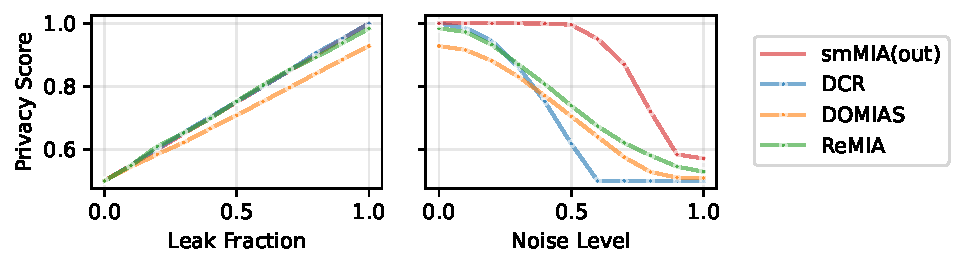
\includegraphics[width=1.0\textwidth]{figures/privacy_risk_vs_leak_fraction_and_noise_level_adult.pdf}
  \caption{Metrics evaluation in risk models (Adult dataset).
  The plots show the privacy risk (AUROC score averaged over 4 seeds) of different metrics for different values of the leak fraction $p$ of the leaky model (left) and noise level $\alpha$ of the noise-based anonymization method (right). All metrics' scores are monotonic with respect to both $p$ and $\alpha$, they follow the maximum achievable by a MIA ($0.5 + \frac{p}{2}$) in the leaky model, while in the anonymized model smMIA(out) score is higher than ReMIA and DOMIAS, that are similar, while DCR performs poorly. Scores inferior to 50\% are clipped to 50\%. Results on the other datasets are reported in Appendix \ref{app:additional_results}.
  }
  \label{leak_fraction_alpha_vs_privacy_adult}
\end{figure}

\paragraph{Privacy-Quality Trade-off.}
We have seen how few models are able to achieve a low privacy risk, but all models that do not present a significant privacy risk generate poor quality synthetic data, both in terms of fidelity and utility. This trade-off between privacy and fidelity is a well-known phenomenon \citep{stadler2022synthetic}. However, there are some models that achieve a better trade-off than others, as we show in Figure \ref{fidelity_vs_privacy_adult}.
Furthermore, in contrast with the conclusions of \citet{stadler2022synthetic} and in line with those of \citet{van2023membership}, we observe that some SDGs are able to achieve a better trade-off than the noise-based anonymization technique, as they are able to achieve a low privacy risk while maintaining a good quality of the synthetic data. More experiments are reported in Appendix \ref{app:additional_results}.
\begin{figure}[t]
  \centering
  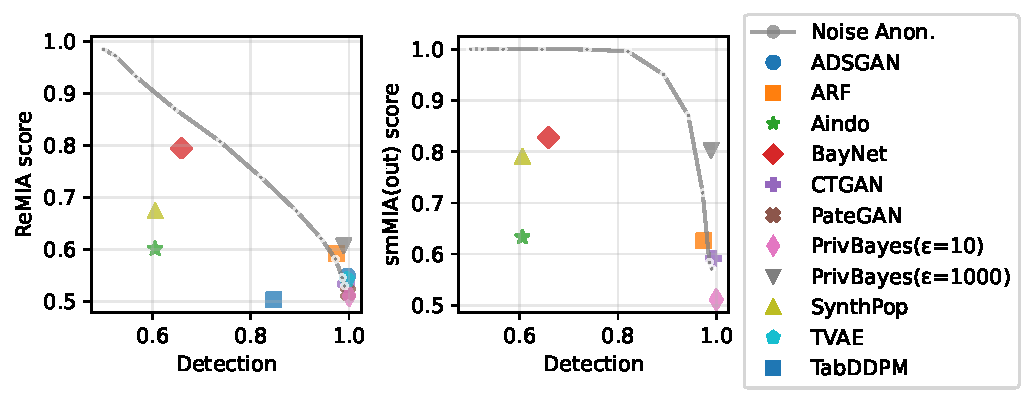
\includegraphics[width=1.0\textwidth]{figures/quality_vs_privacy/adult_detection_vs_remia_sm_mia.pdf}
  \caption{Privacy-fidelity trade-off (Adult dataset). We show the fidelity of the synthetic data in terms of Detection (lower is better) against the privacy scores of ReMIA (left) and smMIA(out) (right). The gray line is the performance of the noise-based anonymization method, meaning that models below the line achieve a better privacy-fidelity trade-off. Results on the other datasets and privacy metrics are reported in Appendix \ref{app:additional_results}.
  }
  \label{fidelity_vs_privacy_adult}
\end{figure}


\paragraph{Efficiency Comparison.}
ReMIA requires only a fraction of the computational time and data of smMIA attacks. Moreover, our method is also more data-efficient than DOMIAS, but it requires training the generative model two times. The overhead time due to training the discriminator is higher than DOMIAS with KDE, but still relatively low.
We show in Table \ref{tab:efficiency_comparison} the comparison of the efficiency of the metrics in terms of computational time, number of models trained and additional data required.
\begin{table}[t]
  \caption{Efficiency comparison. The additional data usage is computed as $\frac{n}{s} - 1$ where $n$ is the total data usage and $s$ is the size of the training datasets. The overhead time is the total time required for running the metric excluding the training of the SDGs. In both cases we report the range of values if they differ across experiments. In the case of smMIAs $n$ depends on the particular dataset. The wide range in overhead time also depends on the dataset used.}
  \label{tab:efficiency_comparison}
  \centering
  \begin{tabular}{llll}
    \toprule
    Metric & SDG Calls & Additional Data Usage & Overhead Time (s) \\
    \midrule
    DCR & 1 & 1.0 & <0.2 \\
    DOMIAS & 1 & 6.0 & 2.7 - 3.6 \\
    ReMIA(f=0.5) & 2 & 0.5 & 7.8 - 23.0 \\
    ReMIA(f=1.0) & 2 & 1.0 & 8.4 - 23.3 \\
    smMIA & 1200 & 19.6 - 74.0 & 16.4 - 4108.0 \\
    \bottomrule
\end{tabular}

\end{table}
Overall, ReMIA represents a practical alternative to MIAs that values computational and data efficiency while maintaining a high sensitivity to privacy risks.
